\chapter{Selected features \& save as new layer}

\pagestyle{fancy}
\fancyhf{}
\fancyhead[OC]{\leftmark}
\fancyhead[EC]{\rightmark}
%\renewcommand{\footrulewidth}{1pt}
\cfoot{\thepage}

In this section we are going to select a single feature (for this example, the polygon UK) and save it as a separate layer.\\

This is useful because we are only interested in the SW England, and so we can have this smaller layer open in our project - reduce computational time redrawing the base map layer.\\ 

\section{Select a feature}
There are many options available to us to select the polygon for UK.

\begin{enumerate}
	\item 
	Using the map canvas: Use the \textit{Select Feature} icon to select the UK polygon from the map canvas.
	\begin{tabular}{@{}c@{}}
\includegraphics[width=4ex]{images/select_features_by_polygon_icon.png}\end{tabular}
	\item 
	Using the layer's \textit{Attribute table}: Open attribute table \& select row with field \textit{Name} = United Kingdom
	
	\begin{figure}[!h]
		\centering
		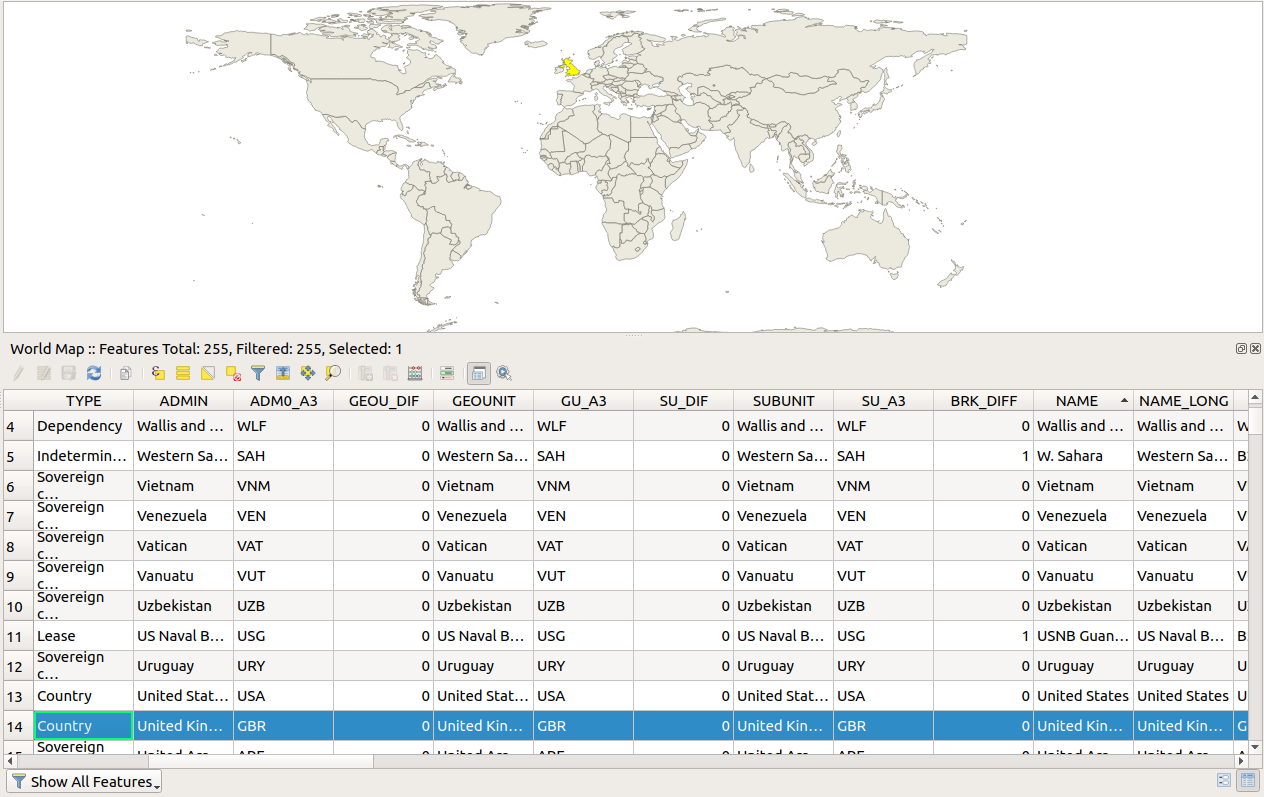
\includegraphics[width=0.5\textwidth]{images/world_select_uk.png}
		\caption{Selecting the feature that corresponds to the UK polygon in the attribute table}
		\label{ft_fig_firstfig3}
	\end{figure}
%%%%%%%%%%%%%%%%%%%
%%EDIT THIS IF WANT IT HERE
%%%%%%%%%%%%%%%%%%%%%
	\item
	Using the \textit{Select \& filter form}: Instead of searching and selecting rows directly in the \textit{Attribute Table}, we can construct our search (build an expression) using a form, that will select our features.
	
	Open the \textit{Attribute Table}. Click	\begin{tabular}{@{}c@{}}
\includegraphics[width=4ex]{images/attribute_table_icon.png}\end{tabular}.\\
	
	Interrogate the data and identify which field contains data in order for us to select those features that are just for UK. We have identified that field "Name" contains the country. Let's select features that contain "United Kingdom" in the field "Name" using the \textit{Select or filter features using form}. \\
	Click the icon at the top of the \textit{Attribute Table}: 
	\begin{tabular}{@{}c@{}}
\includegraphics[width=4ex]{images/select_features_form_icon.png}\end{tabular}.\\
	
	Type \textit{United Kingdom} in the textbox relating to field "Name". QGIS will prompt you with values that are present in the table.\\
	From the dropdown select "Contains".\\
	
	\begin{figure}[!h]
		\centering
		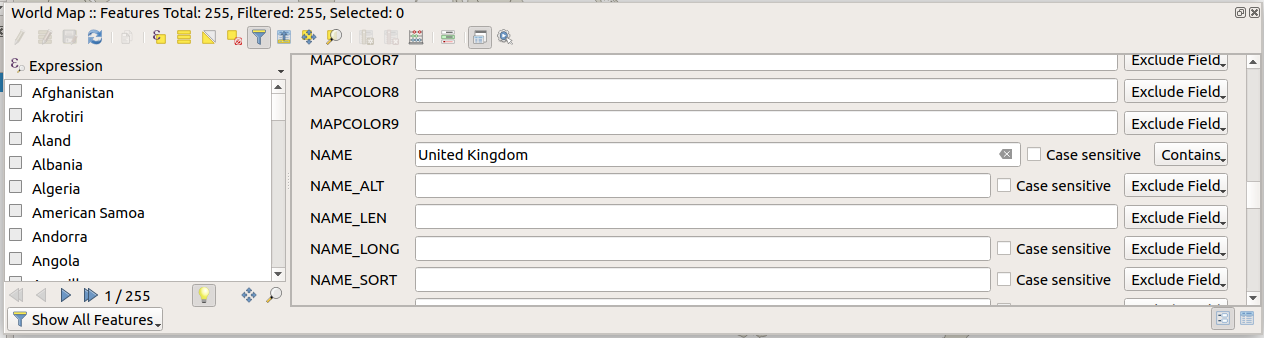
\includegraphics[width=0.7\textwidth]{images/select_filter_features_form_uk.png}
		\caption{Using the Select or Filter features form}
		\label{ft_fig_firstfig3}
	\end{figure}
	
	Scroll to the bottom of this form. If we click the "Filter Features" button in the bottom right we can see the expression that this has built: "NAME" ILIKE '\%United Kingdom\%'
	
	We can toggle between the form view and the attribute table using the buttons in the bottom right
	\begin{tabular}{@{}c@{}}
\includegraphics[width=4ex]{images/form_table_icons.png}\end{tabular}. See in the \textit{Attribute Table} that only 1 features exists for UK.\\
	
	Let's go back to our select \& filter form, click  
	\begin{tabular}{@{}c@{}}
\includegraphics[width=4ex]{images/select_features_form_icon.png}\end{tabular}.\\
	
	At the bottom of the form, now click the "Select Features" button on the bottom. Look at the map. See that UK is yellow (these are the selected polygons). Can zoom or pan the map to them using the \textit{Zoom map to selection} icon
	\begin{tabular}{@{}c@{}}
\includegraphics[width=4ex]{images/zoom_map_to_selection_icon.png}\end{tabular}
	and the \textit{Pan map to selection} icon
	\begin{tabular}{@{}c@{}}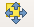
\includegraphics[width=4ex]{images/pan_map_to_selection_icon.png}\end{tabular}
	
	\item 
	Write expression ()
	
	This allows for more complex selections to be made. Once we are familiar with the expressions we can type it directly in. Click the \textit{Select by expression} icon: 
	\begin{tabular}{@{}c@{}}
\includegraphics[width=4ex]{images/select_by_expression_icon.png}\end{tabular}.\\
	
	And fill in the expression in the LHS pane, using the middle pane for prompts ("Field and Values" and "Operators" are very useful).
	
	\begin{figure}[!h]
		\centering
		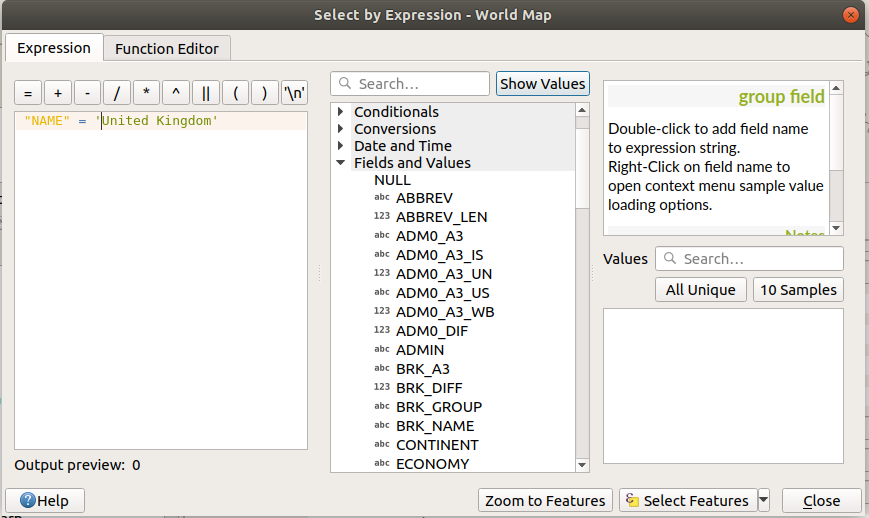
\includegraphics[width=0.6\textwidth]{images/select_by_expression_form_uk.png}
		\caption{Using the Select by Expression form, to select the UK feature}
		\label{ft_fig_firstfig3}
	\end{figure}
	
	%%%%%%%%%%%%%%%%%%%%%
	%%EDIT THIS IF WANT IT HERE
	%%%%%%%%%%%%%%%%%%%%%
	
\end{enumerate}

%Open attribute table.

%Select on UK only


%Or use clicky tools to select.

%("NAME_SORT" = 'United Kingdom')
\null\newpage
\subsection{Save selected feature as a new feature layer}
In the \textit{Layers Panel} right click on the layer's name and select Export $\rightarrow$ Save selected features as...\\

\textbf{Format}: ESRI Shapefile\\
\textbf{File name}: your choice (click on \begin{tabular}{@{}c@{}}
\includegraphics[width=4ex]{images/three_dots_button.png}\end{tabular} to choose destination folder)\\
\textbf{CRS}: leave as default, unless you know something else! \\
Keep "Save only selected features" checked. \\
Keep "Add saved file to map" checked. \\
\textbf{OK}\\

\begin{figure}[!h]
	\centering
	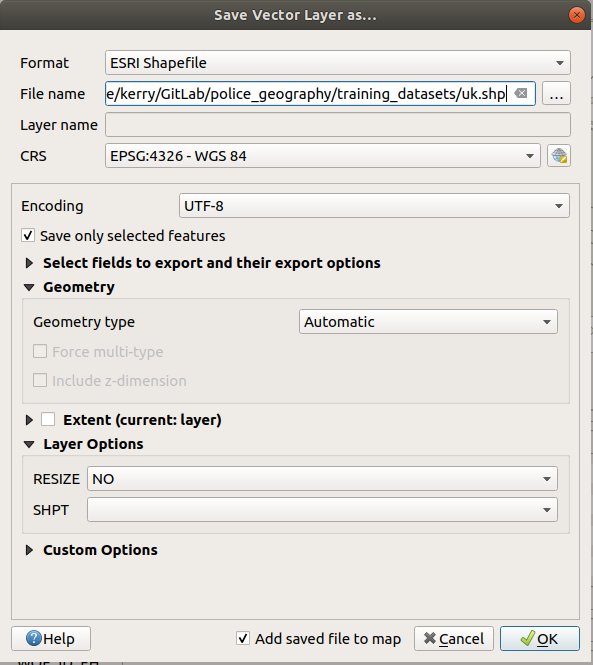
\includegraphics[width=0.6\textwidth]{images/save_as_vector_layer_form.png}%save_vector_layer_form.png}
	\caption{The window for Save Vector Layer as...}
	\label{ft_fig_firstfig3}
\end{figure}

Can see our new layer in the \textit{Layers Panel} and on the map canvas.\\

Within the \textit{Layers Panel} can select and deselect which of these two layers to have visible on map canvas (use the checked boxes), and the order of the layers (drag and drop layer name within layer panel).\\

Can now delete the World layer (on layer name in \textit{Layers panel} right click $\rightarrow$ \textit{Remove layer...}).